%%%%%%%%%%%%%%%%%%%%%%%%%%%%%%%%%%%%%%%%%
% Beamer Presentation
% LaTeX Template
% Version 1.0 (10/11/12)
%
% This template has been downloaded from:
% http://www.LaTeXTemplates.com
%
% License:
% CC BY-NC-SA 3.0 (http://creativecommons.org/licenses/by-nc-sa/3.0/)
%
%%%%%%%%%%%%%%%%%%%%%%%%%%%%%%%%%%%%%%%%%

%----------------------------------------------------------------------------------------
%	PACKAGES AND THEMES
%----------------------------------------------------------------------------------------

\documentclass{beamer}

\mode<presentation> {

% The Beamer class comes with a number of default slide themes
% which change the colors and layouts of slides. Below this is a list
% of all the themes, uncomment each in turn to see what they look like.

%\usetheme{default}
%\usetheme{AnnArbor}
%\usetheme{Antibes}
%\usetheme{Bergen}
%\usetheme{Berkeley}
%\usetheme{Berlin}
%\usetheme{Boadilla}
%\usetheme{CambridgeUS}
%\usetheme{Copenhagen}
%\usetheme{Darmstadt}
%\usetheme{Dresden}
%\usetheme{Frankfurt}
%\usetheme{Goettingen}
%\usetheme{Hannover}
%\usetheme{Ilmenau}
%\usetheme{JuanLesPins}
%\usetheme{Luebeck}
%\usetheme{Madrid}
%\usetheme{Malmoe}
%\usetheme{Marburg}
\usetheme{Montpellier}
%\usetheme{PaloAlto}
%\usetheme{Pittsburgh}
%\usetheme{Rochester}
%\usetheme{Singapore}
%\usetheme{Szeged}
%\usetheme{Warsaw}

% As well as themes, the Beamer class has a number of color themes
% for any slide theme. Uncomment each of these in turn to see how it
% changes the colors of your current slide theme.

%\usecolortheme{albatross}
%\usecolortheme{beaver}
%\usecolortheme{beetle}
%\usecolortheme{crane}
%\usecolortheme{dolphin}
%\usecolortheme{dove} %this seems cool
%\usecolortheme{fly}
%\usecolortheme{lily}
%\usecolortheme{orchid} %this is original
\usecolortheme{rose} % this one is also ok, maybe #1
%\usecolortheme{seagull}
%\usecolortheme{seahorse}
%\usecolortheme{whale}
%\usecolortheme{wolverine}

%\setbeamertemplate{footline} % To remove the footer line in all slides uncomment this line
%\setbeamertemplate{footline}[page number] % To replace the footer line in all slides with a simple slide count uncomment this line

\setbeamertemplate{navigation symbols}{} % To remove the navigation symbols from the bottom of all slides uncomment this line
}

\usepackage{booktabs} % Allows the use of \toprule, \midrule and \bottomrule in tables
\usepackage[utf8]{inputenc}
\usepackage[dvipdfmx]{graphicx} 
\usepackage{bmpsize}
\usepackage{grffile}
%----------------------------------------------------------------------------------------
%	TITLE PAGE
%----------------------------------------------------------------------------------------

\title[BFP Tools]{Profiling with BPF tools} % The short title appears at the bottom of every slide, the full title is only on the title page

\author{Piotr Wieleba} % Your name
\institute[DataArt] % Your institution as it will appear on the bottom of every slide, may be shorthand to save space
{
DataArt\\ % Your institution for the title page
\medskip
\textit{piotr.wieleba@dataart.com} % Your email address
}
\date{\today} % Date, can be changed to a custom date

\begin{document}

\begin{frame}
\titlepage % Print the title page as the first slide
\end{frame}

%\begin{frame}
%\frametitle{Hello}
%\begin{itemize}
%\item<1-> Work in Java/JVM centric technologies for over 11 years
%\item<2-> Currently in DataArt Lublin
%\item<3-> Worked in different domains (education, health care, finance, retail)
%\item<4-> Mostly programming but also been doing a little bit of SRE
%\end{itemize}
%\end{frame}

\begin{frame}
\frametitle{Overview} % Table of contents slide, comment this block out to remove it
\tableofcontents % Throughout your presentation, if you choose to use \section{} and \subsection{} commands, these will automatically be printed on this slide as an overview of your presentation
\end{frame}

%----------------------------------------------------------------------------------------
%	PRESENTATION SLIDES
%----------------------------------------------------------------------------------------

%------------------------------------------------
\section{Introduction} % Sections can be created in order to organize your presentation into discrete blocks, all sections and subsections are automatically printed in the table of contents as an overview of the talk
%------------------------------------------------
\subsection{Basic Terms}

\begin{frame}
  \begin{block}{Tracing}
    \begin{itemize}
      \item<+-> Typically it's an event-based recording.  Big volume require post-processing.
      \item<+-> Some tracers doesn't record events but rather display, periodicaly updated, statistics. Tracers are: \emph{strace}, \emph{top}, \emph{tcpdump}. 
    \end{itemize}
  \end{block}
\end{frame}


\begin{frame}
  \begin{block}{Snooping}
    \begin{itemize}
      \item On Solaris tracer was called \emph{snoop}, that's the reason why we can find bpf based tracers that have snoop in name (execsnoop, opensoop, biosnoop).
    \end{itemize}
  \end{block}
\end{frame}


\begin{frame}
  \begin{block}{Sampling/Profiling}
    \begin{itemize}
      \item<+-> Analyze part of measurements to show coarse grain picture of the system
      \item<+-> Performance overhead can be lower than for tracers
      \item<+-> Samples can be taken once every n miliseconds or n times per second 
    \end{itemize}
  \end{block} 
\end{frame}


\begin{frame}
  \begin{block}{Observability}
    \begin{itemize}
      \item<+-> Reasoning about the system through observation
      \item<+-> BPF tools are observability tools including tracers, samplers
      \item<+-> Benchmarks are not observability tools as they perform predefined work. This doesn't show actual system state
    \end{itemize}
  \end{block} 
\end{frame}


\subsection{BPF} % A subsection can be created just before a set of slides with a common theme to further break down your presentation into chunks

\begin{frame}
\frametitle{History}
\begin{itemize}
\item<1->
BPF (Berkeley Packet Filter)

A minimal instruction set that can be used to filter packets before they are seen by an application such
as tcpdump
\item<2->
In 2014 Alexei Starovoitov created extend BPF so it could be use in wide areas.
He turned BPF into a general-purpose virtual machine, that can be used for a variety of things,
including the creation of advanced performance analysis tools.
\item<3-> Nowdays BPF means actually eBPF
\end{itemize}
\end{frame}

\begin{frame}
  \frametitle{How BPF looks like?}
  \begin{itemize}
    \item<1-> BPF code is similar to bytecode or simple assembly language
    \item<2-> It's rather low level concept designed to be emmited by higher level tools
    \item<3-> {\scriptsize \texttt{\# bpftrace -e 'tracepoint:syscalls:sys\_enter\_exec* \{ @[comm, pid]=count();\}' }}
		\begin{block}{\scriptsize \texttt{\# bpftool prog dump xlated id 4}}
      {\texttt 
			 0: (b7) r1 = 0

			 1: (7b) *(u64 *)(r10 -8) = r1

			 2: (7b) *(u64 *)(r10 -16) = r1

			 3: (bf) r1 = r10

			 4: (07) r1 += -16

			 5: (b7) r2 = 16

			 6: (85) call bpf\_get\_current\_comm\#119536
			 
			 ................
		  }
      \end{block}
  \end{itemize}
\end{frame}

\begin{frame}
  \frametitle{What makes BPF based tools sufficient for analysis in production}
  \begin{itemize}
    \item<1-> Efficient and production safe 
		\item<2-> Build-in into kernel
    \item<3-> No need to add new kernel modules(verifier doesn't allow code that run kernel panic)
		\item<4-> No need to copy every event from kernelspace to userspace 
	\end{itemize}
\end{frame}

\subsection{Instrumentation}

\begin{frame}
  \frametitle{Dynamic Instrumentation kprobes}
  \begin{itemize}
    \item<1-> kprobes can create instrumentation events for any kernel function, and it can instrument instructions within functions

		\item<2-> kprobe and kretprobe allows to calculate the duration of a function 
		\item<3-> in bpftrace kprobes starts with 'kprobe:' or simple 'k:'
    \item<4-> breakepoint instruction int3 or jmp is set in place of target function address and is removed when no longer needed
    \item<5-> {\scriptsize \texttt{\# bpftrace -l 'kprobe:*'}}
	\end{itemize}	
\end{frame}

\begin{frame}
  \frametitle{Dynamic Instrumentation uprobes}
  \begin{itemize}
    \item<1-> uprobes are similar to kprobes but are designed to instrument user-space processes
		\item<2-> similar there is uretprobe
		\item<3-> in bpftrace uprobes starts with 'uprobe:' or simple 'u:'
		\item<4-> can be use to instrument libraries
    \item<5-> {\scriptsize \texttt{\# bpftrace -l 'uprobe:/lib/x86\_64-linux-gnu/libc.so.6' }}
	\end{itemize}	
\end{frame}

\begin{frame}
  \frametitle{Static Instrumentation}
	\begin{itemize}
	  \item<1-> Dynamic instrumentation can instrument functions. Name of the function can change or can be inlined so script can stop working with new version of the library/kernel
		\item<2-> Static instrumentation rely on stable event names not function names
		\item<3-> Downside is that SI is harder to maintenance
		\item<4-> Static kernel instrumentation $\Rightarrow$ tracepoints
		\item<5-> Static user-space instrumentation $\Rightarrow$ USDT user-level statically defined tracing
	\end{itemize}
\end{frame}

\begin{frame}
  \frametitle{Tracepoint}
  \begin{quotation}
    \small A tracepoint placed in code provides a hook to call a function (probe) that you can provide at runtime. A tracepoint can be “on” (a probe is connected to it) or “off” (no probe is attached). 
   
    \small When a tracepoint is “off” it has no effect, except for adding a tiny time penalty (checking a condition for a branch) and space penalty (adding a few bytes for the function call at the end of the instrumented function and adds a data structure in a separate section). 
  \end{quotation}
\end{frame}


%------------------------------------------------
\subsection{FrontEnd tools for BPF}
\begin{frame}
  \frametitle{BCC (BPF Compiler Collection)}
  \begin{itemize}
    \item<1-> BCC allows to write BPF kernel in C and user interface in Python, Lua or C++
    \item<2-> Instalation provides over 70 ready to use performance analysis tools
    \item<3-> No need to write BCC code by yourself
    \item<4-> opensoop, gethostlatency, biotop, tcpconlat, execsnoop and may other
    \item<5-> ~120 small tools, typically /usr/share/bcc/tools
  \end{itemize}
\end{frame}

\begin{frame}
  \begin{figure}
    \centering
    %\noindent\makebox[\textwidth]{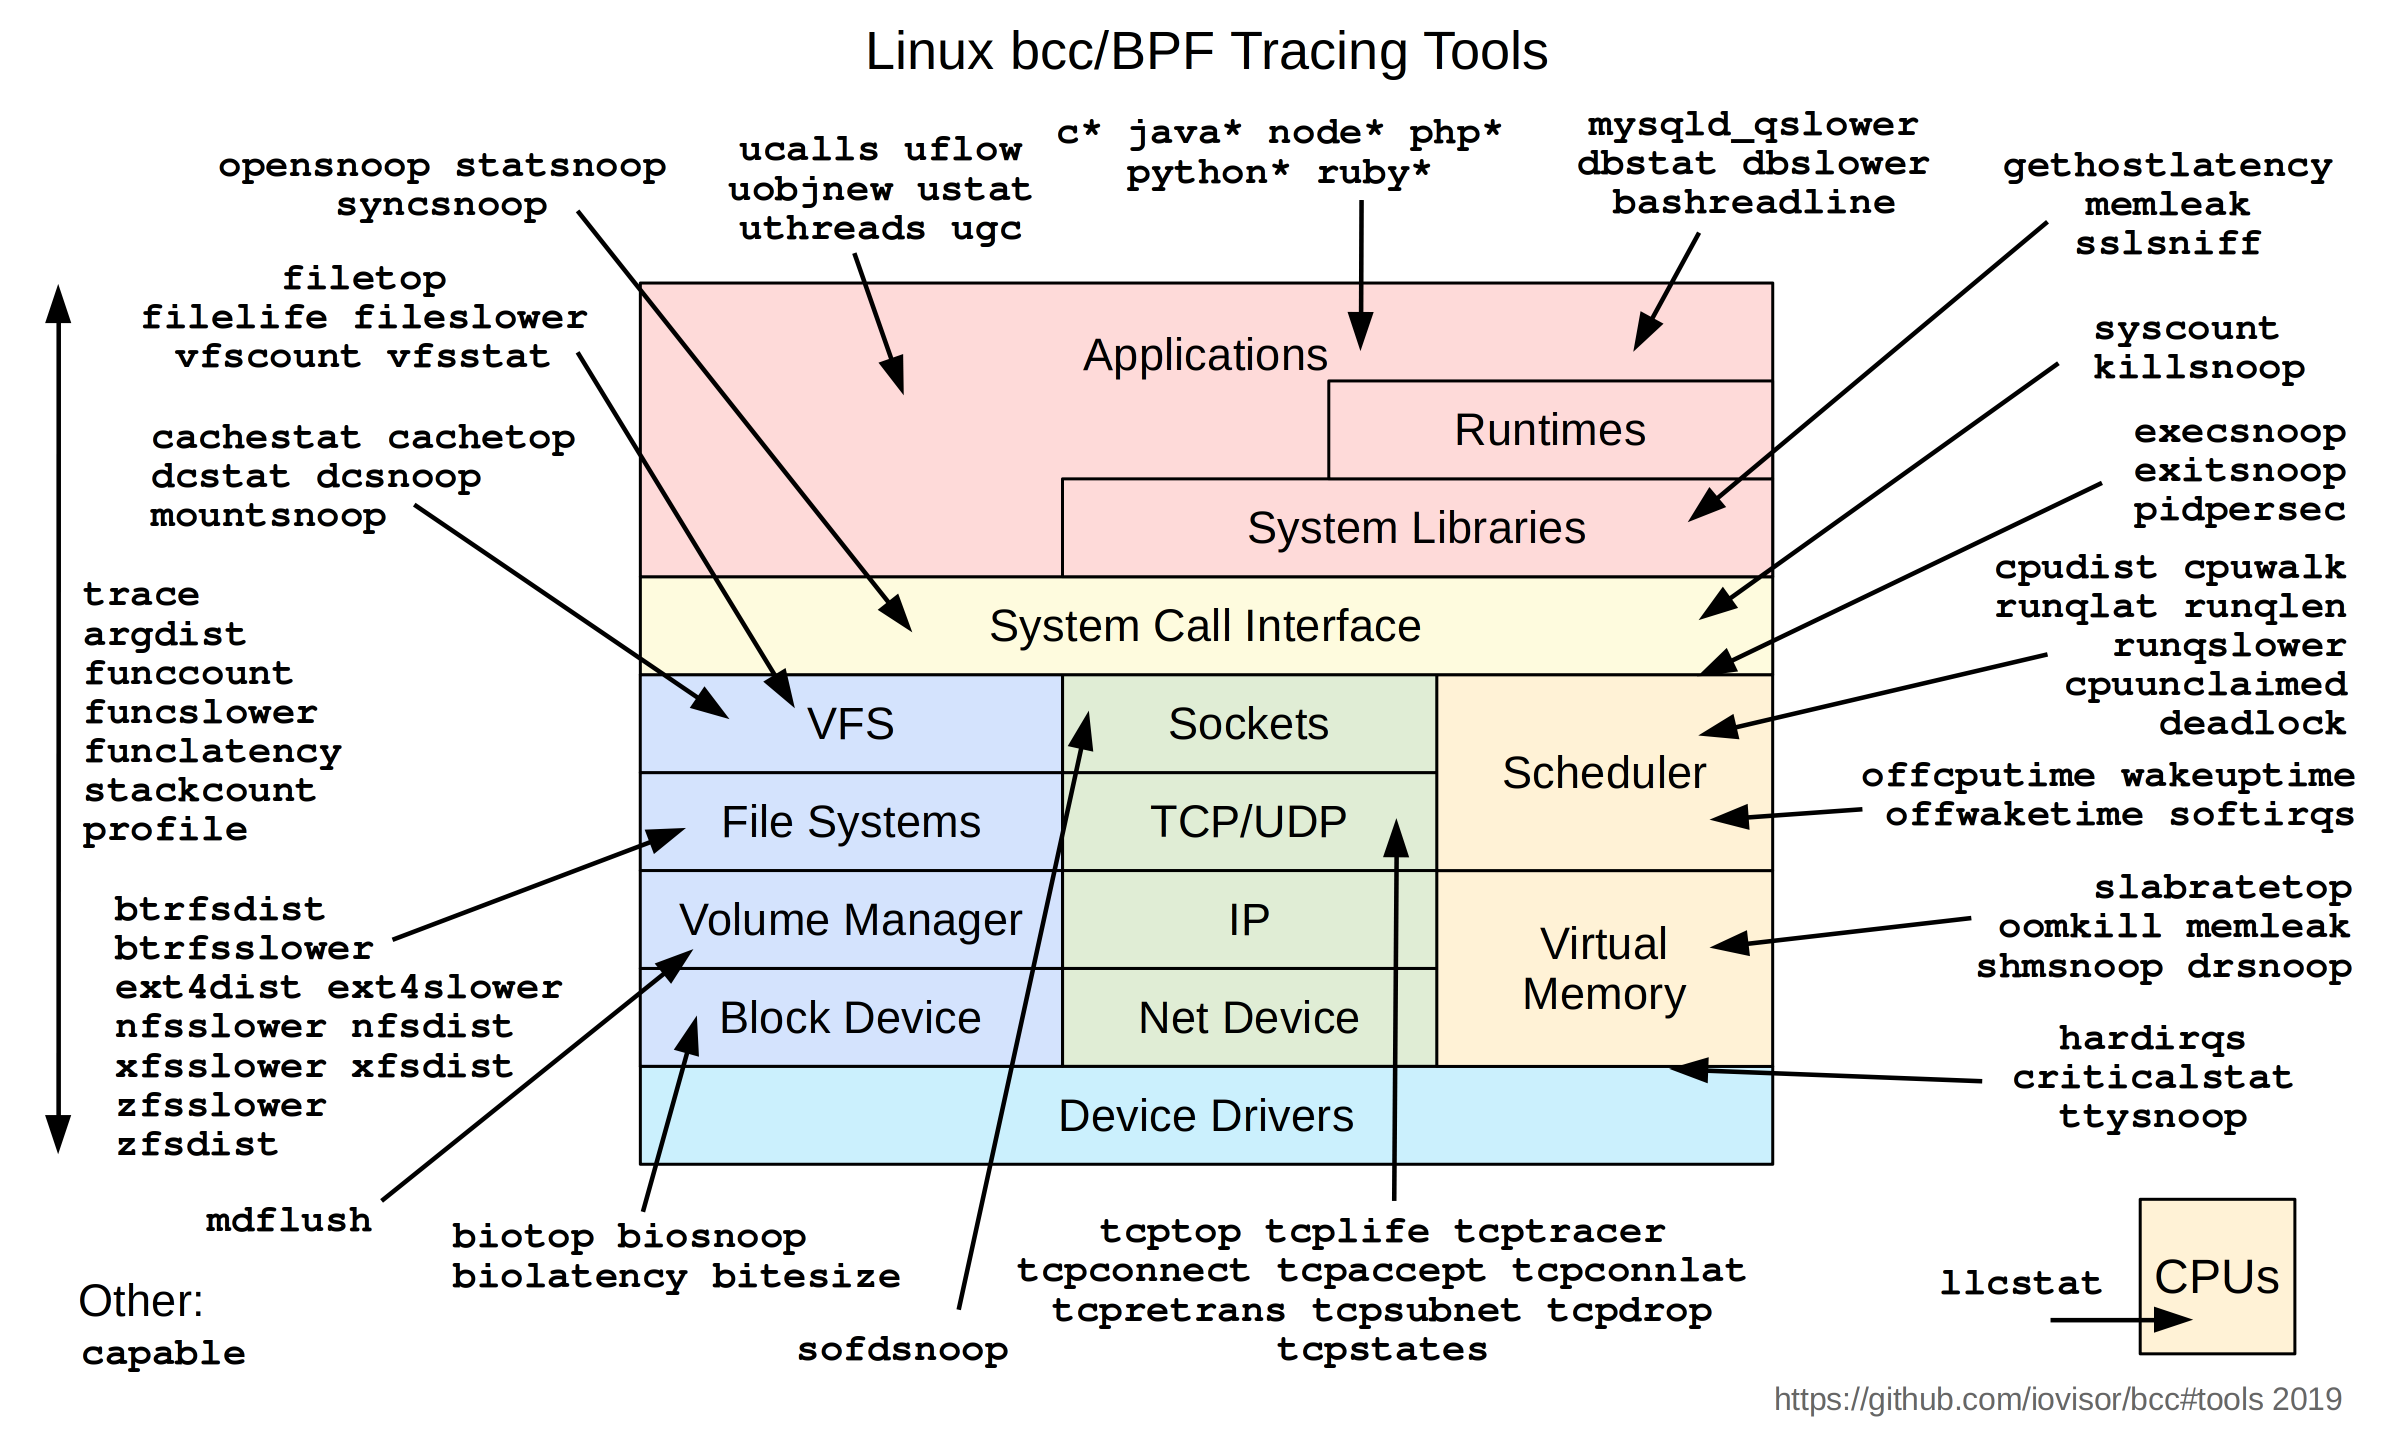
\includegraphics[width=\paperwidth]{bcc_tracing_tools_2019}}
		\noindent\makebox[\textwidth]{\includegraphics[width=\paperwidth]{image.png}}
  \end{figure}
\end{frame}

\begin{frame}
  \frametitle{bpftrace}
  \begin{itemize}
    \item<1-> New frontend tool
    \item<2-> Provide AWK like language to write very specific analytic tools often called oneliners
    \item<3-> More complicated tools can be written as a '.bt' scripts
  \end{itemize}
\end{frame}


%------------------------------------------------
\section{Demo}
%------------------------------------------------

\begin{frame}[fragile] % Need to use the fragile option when verbatim is used in the slide
\frametitle{Example Oneliners}
\begin{example}[Open File]
\begin{verbatim}
bpftrace -e 'tracepoint:syscalls:sys_enter_open 
{ printf("%d %s %s\n", pid, comm, str(args->filename)); }'
\end{verbatim}
\end{example}
\end{frame}


\begin{frame}[fragile] % Need to use the fragile option when verbatim is used in the slide
\frametitle{Example Oneliners}
\begin{example}[Number of times when process open a file]
\begin{verbatim}
sudo bpftrace -e 't:syscalls:sys_enter_open { @[comm, str(args->filename)] = count();}'
\end{verbatim}
\end{example}
\end{frame}


\begin{frame}[fragile] % Need to use the fragile option when verbatim is used in the slide
\frametitle{Example Oneliners}
\begin{example}[Concurrency]
\begin{verbatim}
bpftrace -e 'k:vfs_read { @cpuhash = count(); @hash++; }'
\end{verbatim}
\end{example}
\end{frame}


\begin{frame}
\frametitle{References}
\footnotesize{
\begin{thebibliography}{99} % Beamer does not support BibTeX so references must be inserted manually as below
\bibitem[Gregg, 2020]{p1} Brendan Gregg (2020)
\newblock BPF Performance Tools
\newblock Linux System and Application Observability
\bibitem[iovisor]{p1} \url{https://github.com/iovisor/bcc}
\end{thebibliography}
}
\end{frame}

%------------------------------------------------

\begin{frame}
\Huge{\centerline{The End}}
\end{frame}

%----------------------------------------------------------------------------------------

\end{document} 
